% Appendix B

\chapter{Acceleration Structures} % Main appendix title

\label{AppendixB} % For referencing this appendix elsewhere, use \ref{AppendixA}

\lhead{Appendix B. \emph{Acceleration Structures}} % This is for the header on each page - perhaps a shortened title
%--------------------------------------------------------------------
An \textit{Acceleration} consists of a builder and a traverser. The builder is responsible for collecting input geometry (in most cases, this geometry is the bounding boxes created by geometry nodes' bounding box programs) and computing a data structure that allows a traverser to accelerate a ray-scene intersection query. Builders and traversers are not application-defined programs. Instead, the application chooses an appropriate builder and its corresponding traverser from the table below \citep{Reference6}:\\

\begin{figure}[htbp]
	\centering
		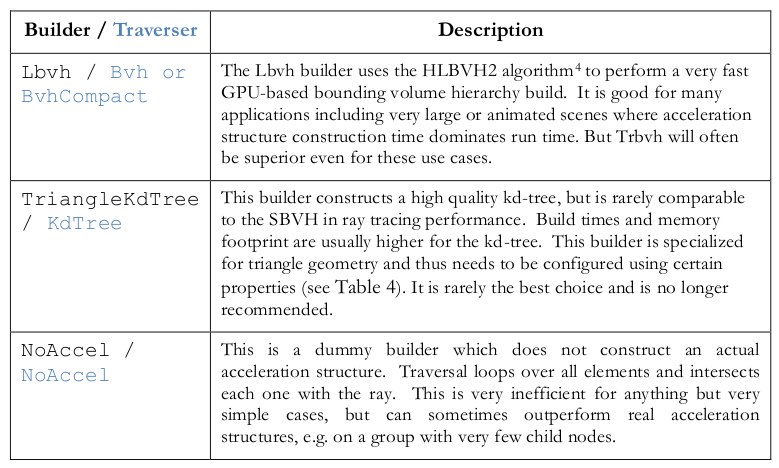
\includegraphics[width=\textwidth,height=\textheight,keepaspectratio]{Figures/acc1.png}
	\caption[Acceleration Structures (1)]{Acceleration Structures (1) \citep{Reference6}.}%{}
	\label{fig:acc1}
\end{figure}
%--------------------------------------------------------------------
\begin{figure}[htbp]
	\centering
		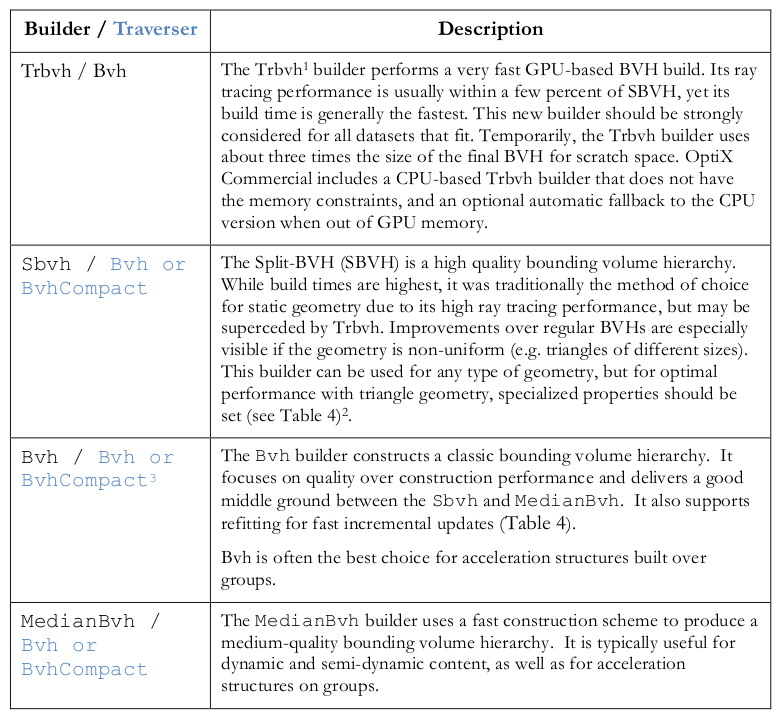
\includegraphics[width=\textwidth,height=\textheight,keepaspectratio]{Figures/acc2.png}
	\caption[Acceleration Structures (2)]{Acceleration Structures (2) \citep{Reference6}.}%{\citep{irprinciple}}
	\label{fig:acc2}
\end{figure}
%--------------------------------------------------------------------
